\documentclass[twoside]{book}

% Packages required by doxygen
\usepackage{fixltx2e}
\usepackage{calc}
\usepackage{doxygen}
\usepackage[export]{adjustbox} % also loads graphicx
\usepackage{graphicx}
\usepackage[utf8]{inputenc}
\usepackage{makeidx}
\usepackage{multicol}
\usepackage{multirow}
\PassOptionsToPackage{warn}{textcomp}
\usepackage{textcomp}
\usepackage[nointegrals]{wasysym}
\usepackage[table]{xcolor}

% Font selection
\usepackage[T1]{fontenc}
\usepackage[scaled=.90]{helvet}
\usepackage{courier}
\usepackage{amssymb}
\usepackage{sectsty}
\renewcommand{\familydefault}{\sfdefault}
\allsectionsfont{%
  \fontseries{bc}\selectfont%
  \color{darkgray}%
}
\renewcommand{\DoxyLabelFont}{%
  \fontseries{bc}\selectfont%
  \color{darkgray}%
}
\newcommand{\+}{\discretionary{\mbox{\scriptsize$\hookleftarrow$}}{}{}}

% Page & text layout
\usepackage{geometry}
\geometry{%
  a4paper,%
  top=2.5cm,%
  bottom=2.5cm,%
  left=2.5cm,%
  right=2.5cm%
}
\tolerance=750
\hfuzz=15pt
\hbadness=750
\setlength{\emergencystretch}{15pt}
\setlength{\parindent}{0cm}
\setlength{\parskip}{3ex plus 2ex minus 2ex}
\makeatletter
\renewcommand{\paragraph}{%
  \@startsection{paragraph}{4}{0ex}{-1.0ex}{1.0ex}{%
    \normalfont\normalsize\bfseries\SS@parafont%
  }%
}
\renewcommand{\subparagraph}{%
  \@startsection{subparagraph}{5}{0ex}{-1.0ex}{1.0ex}{%
    \normalfont\normalsize\bfseries\SS@subparafont%
  }%
}
\makeatother

% Headers & footers
\usepackage{fancyhdr}
\pagestyle{fancyplain}
\fancyhead[LE]{\fancyplain{}{\bfseries\thepage}}
\fancyhead[CE]{\fancyplain{}{}}
\fancyhead[RE]{\fancyplain{}{\bfseries\leftmark}}
\fancyhead[LO]{\fancyplain{}{\bfseries\rightmark}}
\fancyhead[CO]{\fancyplain{}{}}
\fancyhead[RO]{\fancyplain{}{\bfseries\thepage}}
\fancyfoot[LE]{\fancyplain{}{}}
\fancyfoot[CE]{\fancyplain{}{}}
\fancyfoot[RE]{\fancyplain{}{\bfseries\scriptsize Generated by Doxygen }}
\fancyfoot[LO]{\fancyplain{}{\bfseries\scriptsize Generated by Doxygen }}
\fancyfoot[CO]{\fancyplain{}{}}
\fancyfoot[RO]{\fancyplain{}{}}
\renewcommand{\footrulewidth}{0.4pt}
\renewcommand{\chaptermark}[1]{%
  \markboth{#1}{}%
}
\renewcommand{\sectionmark}[1]{%
  \markright{\thesection\ #1}%
}

% Indices & bibliography
\usepackage{natbib}
\usepackage[titles]{tocloft}
\setcounter{tocdepth}{3}
\setcounter{secnumdepth}{5}
\makeindex

% Custom commands
\newcommand{\clearemptydoublepage}{%
  \newpage{\pagestyle{empty}\cleardoublepage}%
}

\usepackage{caption}
\captionsetup{labelsep=space,justification=centering,font={bf},singlelinecheck=off,skip=4pt,position=top}

%===== C O N T E N T S =====

\begin{document}

% Titlepage & ToC
\pagenumbering{alph}
\begin{titlepage}
\vspace*{7cm}
\begin{center}%
{\Large My Project \\[1ex]\large 1.\+0.\+0 }\\
\vspace*{1cm}
{\large Generated by Doxygen 1.8.14}\\
\end{center}
\end{titlepage}
\clearemptydoublepage
\pagenumbering{roman}
\tableofcontents
\clearemptydoublepage
\pagenumbering{arabic}

%--- Begin generated contents ---
\chapter{Hierarchical Index}
\section{Class Hierarchy}
This inheritance list is sorted roughly, but not completely, alphabetically\+:\begin{DoxyCompactList}
\item \contentsline{section}{Figura\+Geometrica}{\pageref{class_figura_geometrica}}{}
\begin{DoxyCompactList}
\item \contentsline{section}{Circulo}{\pageref{class_circulo}}{}
\item \contentsline{section}{Reta}{\pageref{class_reta}}{}
\item \contentsline{section}{Retangulo}{\pageref{class_retangulo}}{}
\end{DoxyCompactList}
\item \contentsline{section}{Screen}{\pageref{class_screen}}{}
\end{DoxyCompactList}

\chapter{Class Index}
\section{Class List}
Here are the classes, structs, unions and interfaces with brief descriptions\+:\begin{DoxyCompactList}
\item\contentsline{section}{\textbf{ Circulo} \\*The \doxyref{Circulo}{p.}{class_circulo} class\+: Desenha circulos }{\pageref{class_circulo}}{}
\item\contentsline{section}{\textbf{ Figura\+Geometrica} \\*The \doxyref{Figura\+Geometrica}{p.}{class_figura_geometrica} class\+: Classe abstrata para desenhar figuras geométricas }{\pageref{class_figura_geometrica}}{}
\item\contentsline{section}{\textbf{ Reta} \\*The \doxyref{Reta}{p.}{class_reta} class\+: Desenha uma reta }{\pageref{class_reta}}{}
\item\contentsline{section}{\textbf{ Retangulo} \\*The \doxyref{Retangulo}{p.}{class_retangulo} class\+: Desenha um retângulo }{\pageref{class_retangulo}}{}
\item\contentsline{section}{\textbf{ Screen} \\*The \doxyref{Screen}{p.}{class_screen} class\+: Classe responsável pela construção da tela }{\pageref{class_screen}}{}
\end{DoxyCompactList}

\chapter{Class Documentation}
\section{Circulo Class Reference}
\label{class_circulo}\index{Circulo@{Circulo}}


The \doxyref{Circulo}{p.}{class_circulo} class\+: Desenha circulos.  




{\ttfamily \#include $<$circulo.\+h$>$}

Inheritance diagram for Circulo\+:\begin{figure}[H]
\begin{center}
\leavevmode
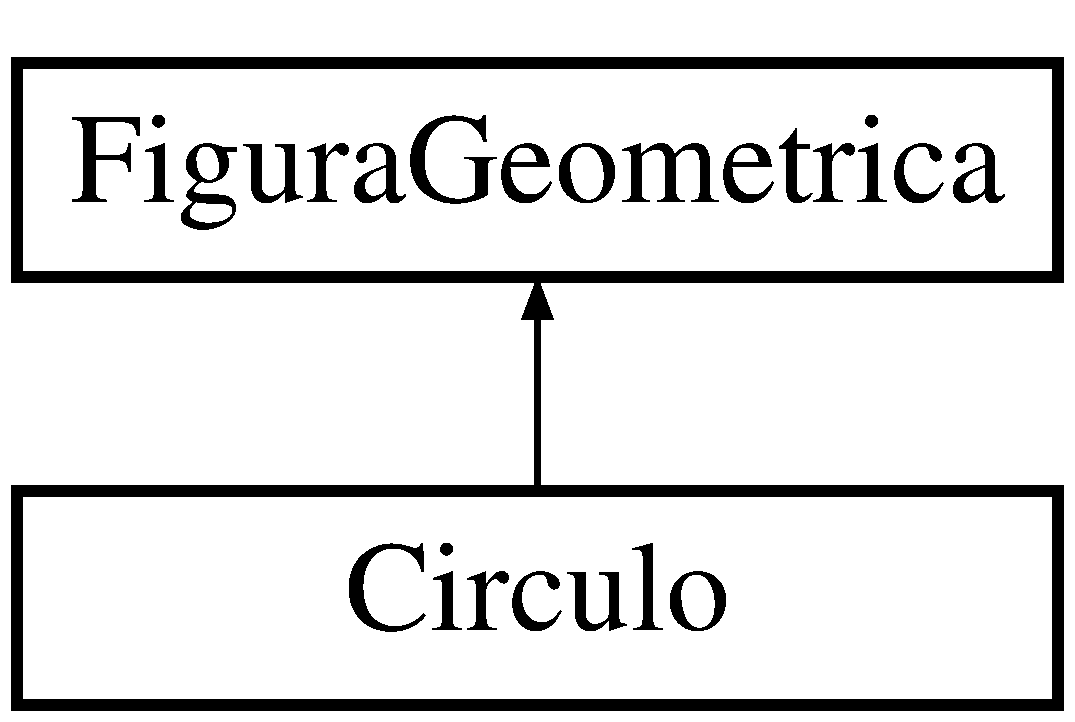
\includegraphics[height=2.000000cm]{class_circulo}
\end{center}
\end{figure}
\subsection*{Public Member Functions}
\begin{DoxyCompactItemize}
\item 
\textbf{ Circulo} (int \+\_\+x0, int \+\_\+y0, int \+\_\+r, int \+\_\+fillmode, char \+\_\+brush)
\begin{DoxyCompactList}\small\item\em \doxyref{Circulo}{p.}{class_circulo}\+: Construtor com argumentos. \end{DoxyCompactList}\item 
void \textbf{ draw} (\textbf{ Screen} \&t)
\begin{DoxyCompactList}\small\item\em draw\+: Desenha um circulo na tela \end{DoxyCompactList}\end{DoxyCompactItemize}
\subsection*{Additional Inherited Members}


\subsection{Detailed Description}
The \doxyref{Circulo}{p.}{class_circulo} class\+: Desenha circulos. 

\subsection{Constructor \& Destructor Documentation}
\mbox{\label{class_circulo_a2029d56d3c7dc5a2c3eecac50400ec65}} 
\index{Circulo@{Circulo}!Circulo@{Circulo}}
\index{Circulo@{Circulo}!Circulo@{Circulo}}
\subsubsection{Circulo()}
{\footnotesize\ttfamily Circulo\+::\+Circulo (\begin{DoxyParamCaption}\item[{int}]{\+\_\+x0,  }\item[{int}]{\+\_\+y0,  }\item[{int}]{\+\_\+r,  }\item[{int}]{\+\_\+fillmode,  }\item[{char}]{\+\_\+brush }\end{DoxyParamCaption})}



\doxyref{Circulo}{p.}{class_circulo}\+: Construtor com argumentos. 


\begin{DoxyParams}{Parameters}
{\em \+\_\+x0} & Coordenada x inicial \\
\hline
{\em \+\_\+y0} & Coordenada y inicial \\
\hline
{\em \+\_\+r} & Raio \\
\hline
{\em \+\_\+fillmode} & Determina se o circulo é preenchido ou não \\
\hline
{\em \+\_\+brush} & Caractere de desenho \\
\hline
\end{DoxyParams}


\subsection{Member Function Documentation}
\mbox{\label{class_circulo_a593787d6e0618c2eded23e8839e7bea6}} 
\index{Circulo@{Circulo}!draw@{draw}}
\index{draw@{draw}!Circulo@{Circulo}}
\subsubsection{draw()}
{\footnotesize\ttfamily void Circulo\+::draw (\begin{DoxyParamCaption}\item[{\textbf{ Screen} \&}]{t }\end{DoxyParamCaption})\hspace{0.3cm}{\ttfamily [virtual]}}



draw\+: Desenha um circulo na tela 


\begin{DoxyParams}{Parameters}
{\em t} & Tela \\
\hline
\end{DoxyParams}


Implements \textbf{ Figura\+Geometrica} \doxyref{}{p.}{class_figura_geometrica_a8ee8dedc060b6059a805ea091aef2c41}.



The documentation for this class was generated from the following files\+:\begin{DoxyCompactItemize}
\item 
circulo.\+h\item 
circulo.\+cpp\end{DoxyCompactItemize}

\section{Figura\+Geometrica Class Reference}
\label{class_figura_geometrica}\index{Figura\+Geometrica@{Figura\+Geometrica}}


The \doxyref{Figura\+Geometrica}{p.}{class_figura_geometrica} class\+: Classe abstrata para desenhar figuras geométricas.  




{\ttfamily \#include $<$figurageometrica.\+h$>$}

Inheritance diagram for Figura\+Geometrica\+:\begin{figure}[H]
\begin{center}
\leavevmode
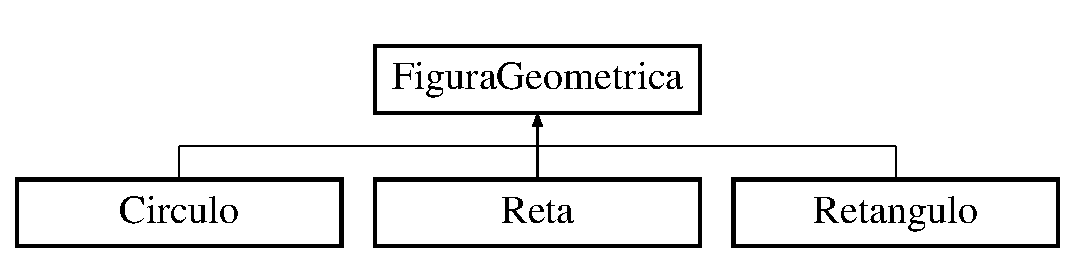
\includegraphics[height=2.000000cm]{class_figura_geometrica}
\end{center}
\end{figure}
\subsection*{Public Member Functions}
\begin{DoxyCompactItemize}
\item 
virtual void \textbf{ draw} (\textbf{ Screen} \&t)=0
\begin{DoxyCompactList}\small\item\em draw\+: Desenha figuras geométricas \end{DoxyCompactList}\end{DoxyCompactItemize}
\subsection*{Public Attributes}
\begin{DoxyCompactItemize}
\item 
\mbox{\label{class_figura_geometrica_a7b835ffcb2f0ef57432167f997c75b8b}} 
char \textbf{ brush}
\begin{DoxyCompactList}\small\item\em brush\+: Caractere de desenho \end{DoxyCompactList}\end{DoxyCompactItemize}


\subsection{Detailed Description}
The \doxyref{Figura\+Geometrica}{p.}{class_figura_geometrica} class\+: Classe abstrata para desenhar figuras geométricas. 

\subsection{Member Function Documentation}
\mbox{\label{class_figura_geometrica_a8ee8dedc060b6059a805ea091aef2c41}} 
\index{Figura\+Geometrica@{Figura\+Geometrica}!draw@{draw}}
\index{draw@{draw}!Figura\+Geometrica@{Figura\+Geometrica}}
\subsubsection{draw()}
{\footnotesize\ttfamily virtual void Figura\+Geometrica\+::draw (\begin{DoxyParamCaption}\item[{\textbf{ Screen} \&}]{t }\end{DoxyParamCaption})\hspace{0.3cm}{\ttfamily [pure virtual]}}



draw\+: Desenha figuras geométricas 


\begin{DoxyParams}{Parameters}
{\em t} & Tela \\
\hline
\end{DoxyParams}


Implemented in \textbf{ Reta} \doxyref{}{p.}{class_reta_ac2e9805183cd474b62bffd8b032cd780}, \textbf{ Circulo} \doxyref{}{p.}{class_circulo_a593787d6e0618c2eded23e8839e7bea6}, and \textbf{ Retangulo} \doxyref{}{p.}{class_retangulo_ac088dd6d3f4f3d3f80363a868c2e74f1}.



The documentation for this class was generated from the following file\+:\begin{DoxyCompactItemize}
\item 
figurageometrica.\+h\end{DoxyCompactItemize}

\section{Reta Class Reference}
\label{class_reta}\index{Reta@{Reta}}


The \doxyref{Reta}{p.}{class_reta} class\+: Desenha uma reta.  




{\ttfamily \#include $<$reta.\+h$>$}

Inheritance diagram for Reta\+:\begin{figure}[H]
\begin{center}
\leavevmode
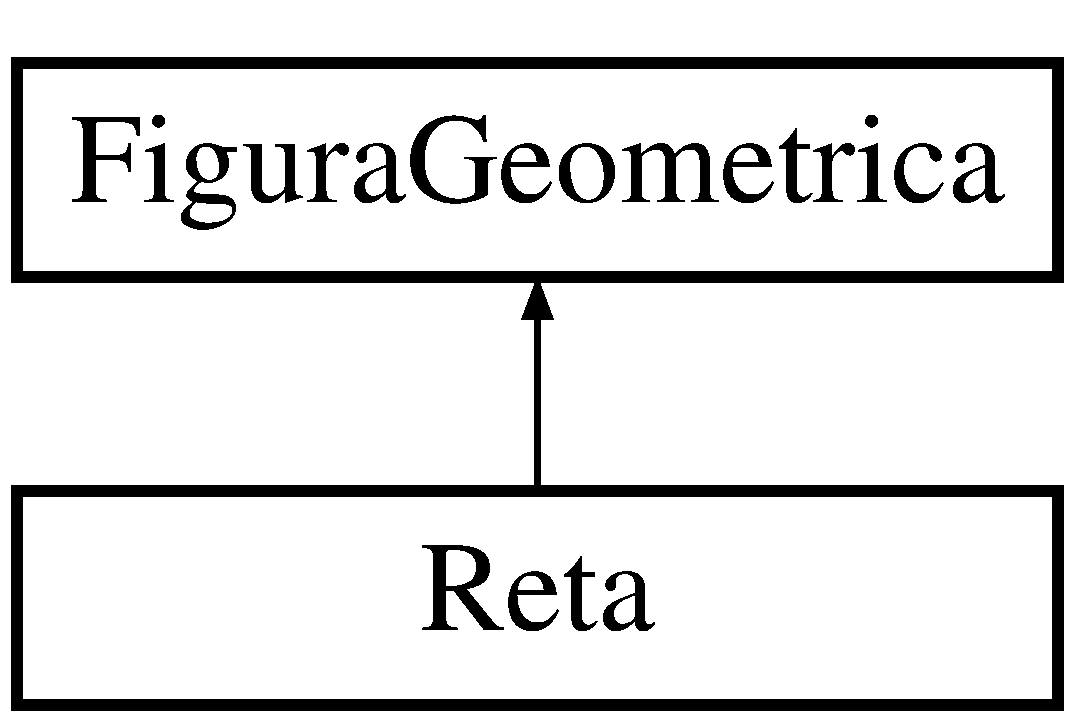
\includegraphics[height=2.000000cm]{class_reta}
\end{center}
\end{figure}
\subsection*{Public Member Functions}
\begin{DoxyCompactItemize}
\item 
\textbf{ Reta} (int \+\_\+x0, int \+\_\+y0, int \+\_\+x1, int \+\_\+y1, char \+\_\+brush)
\begin{DoxyCompactList}\small\item\em \doxyref{Reta}{p.}{class_reta}\+: Construtor com argumentos. \end{DoxyCompactList}\item 
int \textbf{ Sinal} (int x)
\begin{DoxyCompactList}\small\item\em Sinal\+: auxilía draw no desenho da reta. \end{DoxyCompactList}\item 
void \textbf{ draw} (\textbf{ Screen} \&t)
\begin{DoxyCompactList}\small\item\em draw\+: Desenha a reta na tela \end{DoxyCompactList}\end{DoxyCompactItemize}
\subsection*{Additional Inherited Members}


\subsection{Detailed Description}
The \doxyref{Reta}{p.}{class_reta} class\+: Desenha uma reta. 

\subsection{Constructor \& Destructor Documentation}
\mbox{\label{class_reta_a8a02b4b99c3b8cde3c0a6d04b6937ef7}} 
\index{Reta@{Reta}!Reta@{Reta}}
\index{Reta@{Reta}!Reta@{Reta}}
\subsubsection{Reta()}
{\footnotesize\ttfamily Reta\+::\+Reta (\begin{DoxyParamCaption}\item[{int}]{\+\_\+x0,  }\item[{int}]{\+\_\+y0,  }\item[{int}]{\+\_\+x1,  }\item[{int}]{\+\_\+y1,  }\item[{char}]{\+\_\+brush }\end{DoxyParamCaption})}



\doxyref{Reta}{p.}{class_reta}\+: Construtor com argumentos. 


\begin{DoxyParams}{Parameters}
{\em \+\_\+x0} & Coordenada x do ponto inicial \\
\hline
{\em \+\_\+y0} & Coordenada y do ponto inicial \\
\hline
{\em \+\_\+x1} & Coordenada x do ponto final \\
\hline
{\em \+\_\+y1} & Coordenada y do ponto final \\
\hline
{\em \+\_\+brush} & Caractere de desenho \\
\hline
\end{DoxyParams}


\subsection{Member Function Documentation}
\mbox{\label{class_reta_ac2e9805183cd474b62bffd8b032cd780}} 
\index{Reta@{Reta}!draw@{draw}}
\index{draw@{draw}!Reta@{Reta}}
\subsubsection{draw()}
{\footnotesize\ttfamily void Reta\+::draw (\begin{DoxyParamCaption}\item[{\textbf{ Screen} \&}]{t }\end{DoxyParamCaption})\hspace{0.3cm}{\ttfamily [virtual]}}



draw\+: Desenha a reta na tela 


\begin{DoxyParams}{Parameters}
{\em t} & Tela \\
\hline
\end{DoxyParams}


Implements \textbf{ Figura\+Geometrica} \doxyref{}{p.}{class_figura_geometrica_a8ee8dedc060b6059a805ea091aef2c41}.

\mbox{\label{class_reta_a0890517655f27827a827c88850f8984e}} 
\index{Reta@{Reta}!Sinal@{Sinal}}
\index{Sinal@{Sinal}!Reta@{Reta}}
\subsubsection{Sinal()}
{\footnotesize\ttfamily int Reta\+::\+Sinal (\begin{DoxyParamCaption}\item[{int}]{x }\end{DoxyParamCaption})}



Sinal\+: auxilía draw no desenho da reta. 


\begin{DoxyParams}{Parameters}
{\em x} & \\
\hline
\end{DoxyParams}
\begin{DoxyReturn}{Returns}

\end{DoxyReturn}


The documentation for this class was generated from the following files\+:\begin{DoxyCompactItemize}
\item 
reta.\+h\item 
reta.\+cpp\end{DoxyCompactItemize}

\section{Retangulo Class Reference}
\label{class_retangulo}\index{Retangulo@{Retangulo}}


The \doxyref{Retangulo}{p.}{class_retangulo} class\+: Desenha um retângulo.  




{\ttfamily \#include $<$retangulo.\+h$>$}

Inheritance diagram for Retangulo\+:\begin{figure}[H]
\begin{center}
\leavevmode
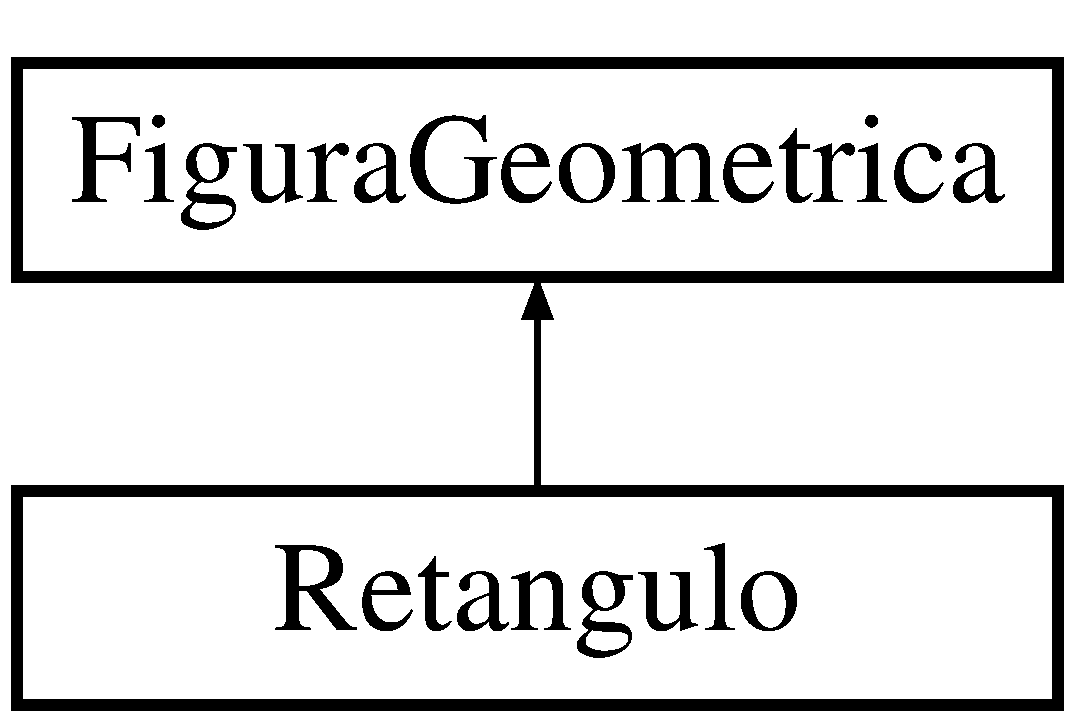
\includegraphics[height=2.000000cm]{class_retangulo}
\end{center}
\end{figure}
\subsection*{Public Member Functions}
\begin{DoxyCompactItemize}
\item 
\textbf{ Retangulo} (int \+\_\+x0, int \+\_\+y0, int \+\_\+larg, int \+\_\+alt, int \+\_\+fillmode, char \+\_\+brush)
\begin{DoxyCompactList}\small\item\em \doxyref{Retangulo}{p.}{class_retangulo}\+: Construtor com argumentos. \end{DoxyCompactList}\item 
void \textbf{ draw} (\textbf{ Screen} \&t)
\begin{DoxyCompactList}\small\item\em draw\+: Desenha um retâmgulo na tela \end{DoxyCompactList}\end{DoxyCompactItemize}
\subsection*{Additional Inherited Members}


\subsection{Detailed Description}
The \doxyref{Retangulo}{p.}{class_retangulo} class\+: Desenha um retângulo. 

\subsection{Constructor \& Destructor Documentation}
\mbox{\label{class_retangulo_abd3f3094751f5500de5407c8e2c3a271}} 
\index{Retangulo@{Retangulo}!Retangulo@{Retangulo}}
\index{Retangulo@{Retangulo}!Retangulo@{Retangulo}}
\subsubsection{Retangulo()}
{\footnotesize\ttfamily Retangulo\+::\+Retangulo (\begin{DoxyParamCaption}\item[{int}]{\+\_\+x0,  }\item[{int}]{\+\_\+y0,  }\item[{int}]{\+\_\+larg,  }\item[{int}]{\+\_\+alt,  }\item[{int}]{\+\_\+fillmode,  }\item[{char}]{\+\_\+brush }\end{DoxyParamCaption})}



\doxyref{Retangulo}{p.}{class_retangulo}\+: Construtor com argumentos. 


\begin{DoxyParams}{Parameters}
{\em \+\_\+x0} & Coordenada x do ponto inicial \\
\hline
{\em \+\_\+y0} & Coordenada y do ponto inicial \\
\hline
{\em \+\_\+larg} & Largura \\
\hline
{\em \+\_\+alt} & Altura \\
\hline
{\em \+\_\+fillmode} & Determina se o retângulo é preenchido ou não \\
\hline
{\em \+\_\+brush} & Caractere de desenho \\
\hline
\end{DoxyParams}


\subsection{Member Function Documentation}
\mbox{\label{class_retangulo_ac088dd6d3f4f3d3f80363a868c2e74f1}} 
\index{Retangulo@{Retangulo}!draw@{draw}}
\index{draw@{draw}!Retangulo@{Retangulo}}
\subsubsection{draw()}
{\footnotesize\ttfamily void Retangulo\+::draw (\begin{DoxyParamCaption}\item[{\textbf{ Screen} \&}]{t }\end{DoxyParamCaption})\hspace{0.3cm}{\ttfamily [virtual]}}



draw\+: Desenha um retâmgulo na tela 


\begin{DoxyParams}{Parameters}
{\em t} & Tela \\
\hline
\end{DoxyParams}


Implements \textbf{ Figura\+Geometrica} \doxyref{}{p.}{class_figura_geometrica_a8ee8dedc060b6059a805ea091aef2c41}.



The documentation for this class was generated from the following files\+:\begin{DoxyCompactItemize}
\item 
retangulo.\+h\item 
retangulo.\+cpp\end{DoxyCompactItemize}

\section{Screen Class Reference}
\label{class_screen}\index{Screen@{Screen}}


The \doxyref{Screen}{p.}{class_screen} class\+: Classe responsável pela construção da tela.  




{\ttfamily \#include $<$screen.\+h$>$}

\subsection*{Public Member Functions}
\begin{DoxyCompactItemize}
\item 
\textbf{ Screen} (int \+\_\+nlin=40, int \+\_\+ncol=40)
\begin{DoxyCompactList}\small\item\em \doxyref{Screen}{p.}{class_screen}\+: Construtor com argumentos. \end{DoxyCompactList}\item 
void \textbf{ set\+Screen} (int lin, int col)
\begin{DoxyCompactList}\small\item\em set\+Screen\+: Seta a matriz na tela \end{DoxyCompactList}\item 
void \textbf{ set\+Pixel} (int x, int y)
\begin{DoxyCompactList}\small\item\em set\+Pixel\+: Desenha um pixel da matriz usando o caratere guardado em brush \end{DoxyCompactList}\item 
\mbox{\label{class_screen_a35e74266b2a04e37b354ceff7a5f1031}} 
void \textbf{ clear} ()
\begin{DoxyCompactList}\small\item\em clear\+: Limpa a tela \end{DoxyCompactList}\item 
void \textbf{ set\+Brush} (char \+\_\+brush)
\begin{DoxyCompactList}\small\item\em set\+Brush\+: Muda o caractere guardado em brush \end{DoxyCompactList}\end{DoxyCompactItemize}
\subsection*{Friends}
\begin{DoxyCompactItemize}
\item 
ostream \& \textbf{ operator$<$$<$} (ostream \&os, \textbf{ Screen} \&t)
\begin{DoxyCompactList}\small\item\em ostream\&\+: envia a tela para um stream de saida \end{DoxyCompactList}\end{DoxyCompactItemize}


\subsection{Detailed Description}
The \doxyref{Screen}{p.}{class_screen} class\+: Classe responsável pela construção da tela. 

\subsection{Constructor \& Destructor Documentation}
\mbox{\label{class_screen_ab3b8c9aeb1cf687c80c98397184f2293}} 
\index{Screen@{Screen}!Screen@{Screen}}
\index{Screen@{Screen}!Screen@{Screen}}
\subsubsection{Screen()}
{\footnotesize\ttfamily Screen\+::\+Screen (\begin{DoxyParamCaption}\item[{int}]{\+\_\+nlin = {\ttfamily 40},  }\item[{int}]{\+\_\+ncol = {\ttfamily 40} }\end{DoxyParamCaption})}



\doxyref{Screen}{p.}{class_screen}\+: Construtor com argumentos. 


\begin{DoxyParams}{Parameters}
{\em \+\_\+nlin} & Numero de linhas da tela \\
\hline
{\em \+\_\+ncol} & Numero de colunas da tela \\
\hline
\end{DoxyParams}


\subsection{Member Function Documentation}
\mbox{\label{class_screen_aebc4eb6cb5acf15a0f04c1494622ab23}} 
\index{Screen@{Screen}!set\+Brush@{set\+Brush}}
\index{set\+Brush@{set\+Brush}!Screen@{Screen}}
\subsubsection{set\+Brush()}
{\footnotesize\ttfamily void Screen\+::set\+Brush (\begin{DoxyParamCaption}\item[{char}]{\+\_\+brush }\end{DoxyParamCaption})}



set\+Brush\+: Muda o caractere guardado em brush 


\begin{DoxyParams}{Parameters}
{\em \+\_\+brush} & Caractere de desenho \\
\hline
\end{DoxyParams}
\mbox{\label{class_screen_ae6bea81c57a22d226507c3c26fa95ee0}} 
\index{Screen@{Screen}!set\+Pixel@{set\+Pixel}}
\index{set\+Pixel@{set\+Pixel}!Screen@{Screen}}
\subsubsection{set\+Pixel()}
{\footnotesize\ttfamily void Screen\+::set\+Pixel (\begin{DoxyParamCaption}\item[{int}]{x,  }\item[{int}]{y }\end{DoxyParamCaption})}



set\+Pixel\+: Desenha um pixel da matriz usando o caratere guardado em brush 


\begin{DoxyParams}{Parameters}
{\em x} & Coordenada do pixel em x \\
\hline
{\em y} & Coordenada do pixel em y \\
\hline
\end{DoxyParams}
\mbox{\label{class_screen_a13e5457f12f447082d4f7b1e70513be1}} 
\index{Screen@{Screen}!set\+Screen@{set\+Screen}}
\index{set\+Screen@{set\+Screen}!Screen@{Screen}}
\subsubsection{set\+Screen()}
{\footnotesize\ttfamily void Screen\+::set\+Screen (\begin{DoxyParamCaption}\item[{int}]{lin,  }\item[{int}]{col }\end{DoxyParamCaption})}



set\+Screen\+: Seta a matriz na tela 


\begin{DoxyParams}{Parameters}
{\em lin} & Numero de linhas da tela \\
\hline
{\em col} & Numero de colunas da tela \\
\hline
\end{DoxyParams}


\subsection{Friends And Related Function Documentation}
\mbox{\label{class_screen_aab6a2880746bfe1b7964817cc8f0989e}} 
\index{Screen@{Screen}!operator$<$$<$@{operator$<$$<$}}
\index{operator$<$$<$@{operator$<$$<$}!Screen@{Screen}}
\subsubsection{operator$<$$<$}
{\footnotesize\ttfamily ostream\& operator$<$$<$ (\begin{DoxyParamCaption}\item[{ostream \&}]{os,  }\item[{\textbf{ Screen} \&}]{t }\end{DoxyParamCaption})\hspace{0.3cm}{\ttfamily [friend]}}



ostream\&\+: envia a tela para um stream de saida 


\begin{DoxyParams}{Parameters}
{\em os} & \\
\hline
{\em t} & Tela \\
\hline
\end{DoxyParams}
\begin{DoxyReturn}{Returns}

\end{DoxyReturn}


The documentation for this class was generated from the following files\+:\begin{DoxyCompactItemize}
\item 
screen.\+h\item 
screen.\+cpp\end{DoxyCompactItemize}

%--- End generated contents ---

% Index
\backmatter
\newpage
\phantomsection
\clearemptydoublepage
\addcontentsline{toc}{chapter}{Index}
\printindex

\end{document}
